\chapter{Fringe field compensation using solenoids} \label{app-C}

It is worth illuminating the finding from \cite{Holmes2018} that in an otherwise linear lattice, fringe fields tend to eliminate any cross-plane correlations in the beam when the tunes are near the difference resonance $\nu_x \approx \nu_y$. To demonstrate this, a Danilov distribution matched to a linearized version of the SNS ring was generated. Fringe fields were then turned on, and the particles were tracked without space charge. Fig.~\ref{fig:fringe_a} shows the turn-by-turn evolution of the distribution.

\begin{figure}[!p]
    \centering
    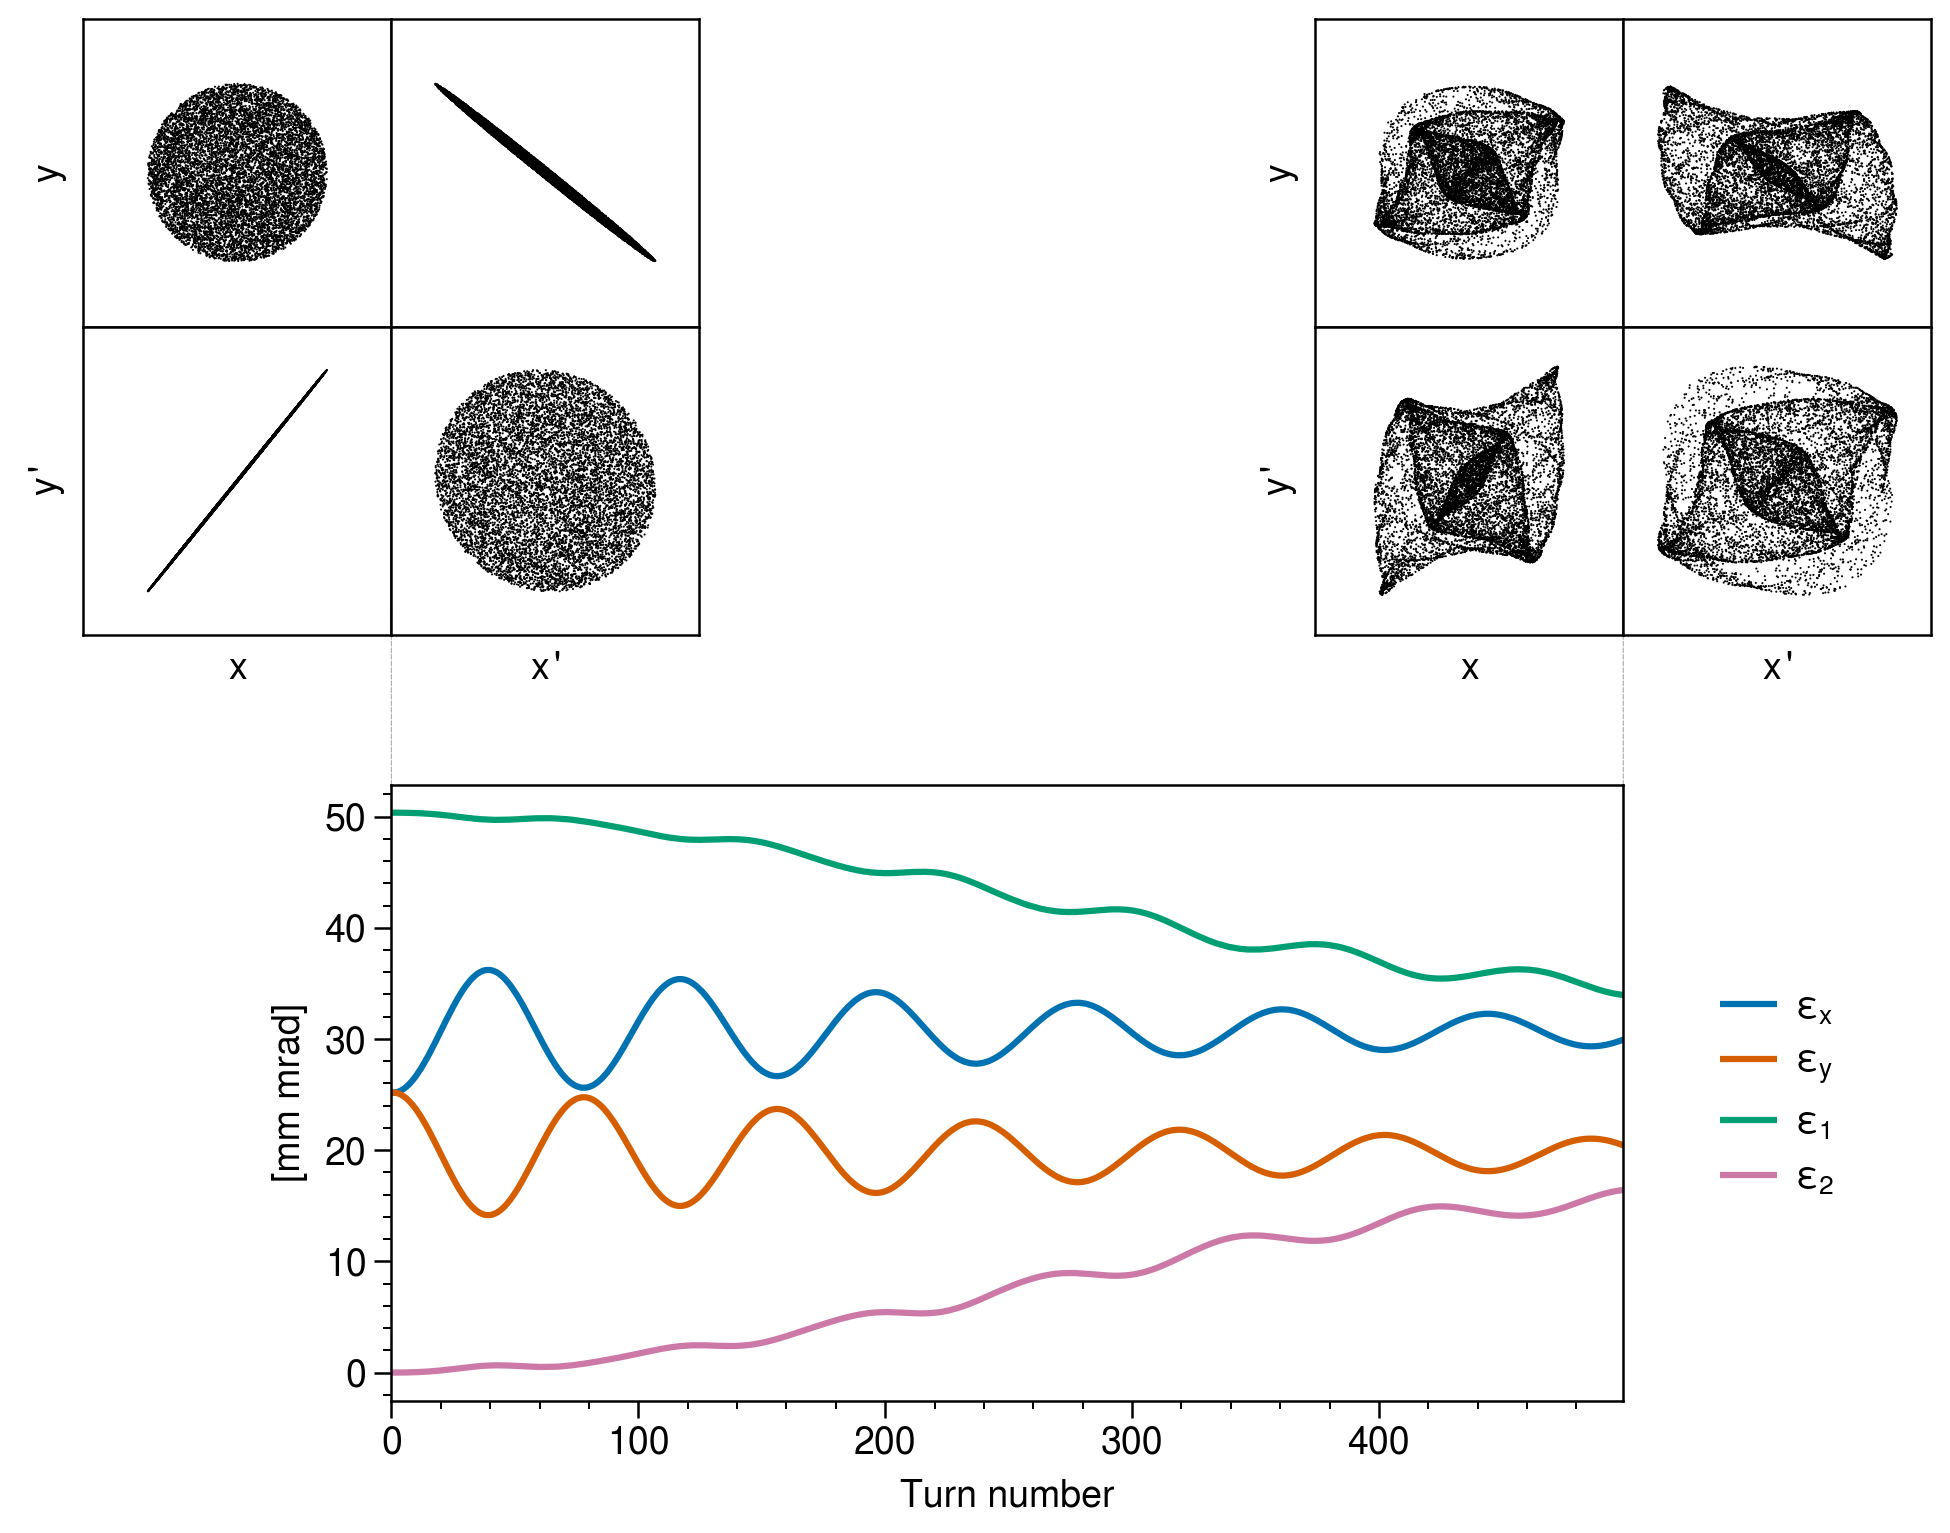
\includegraphics[width=0.7\textwidth]{Images/chapter3/fringe.png}
    \caption{Danilov distribution tracked in the SNS ring. Fringe fields are the only nonlinear external effect.}
    \label{fig:fringe_a}
    \vspace*{3cm}
\end{figure}

\begin{figure}[!p]
    \centering
    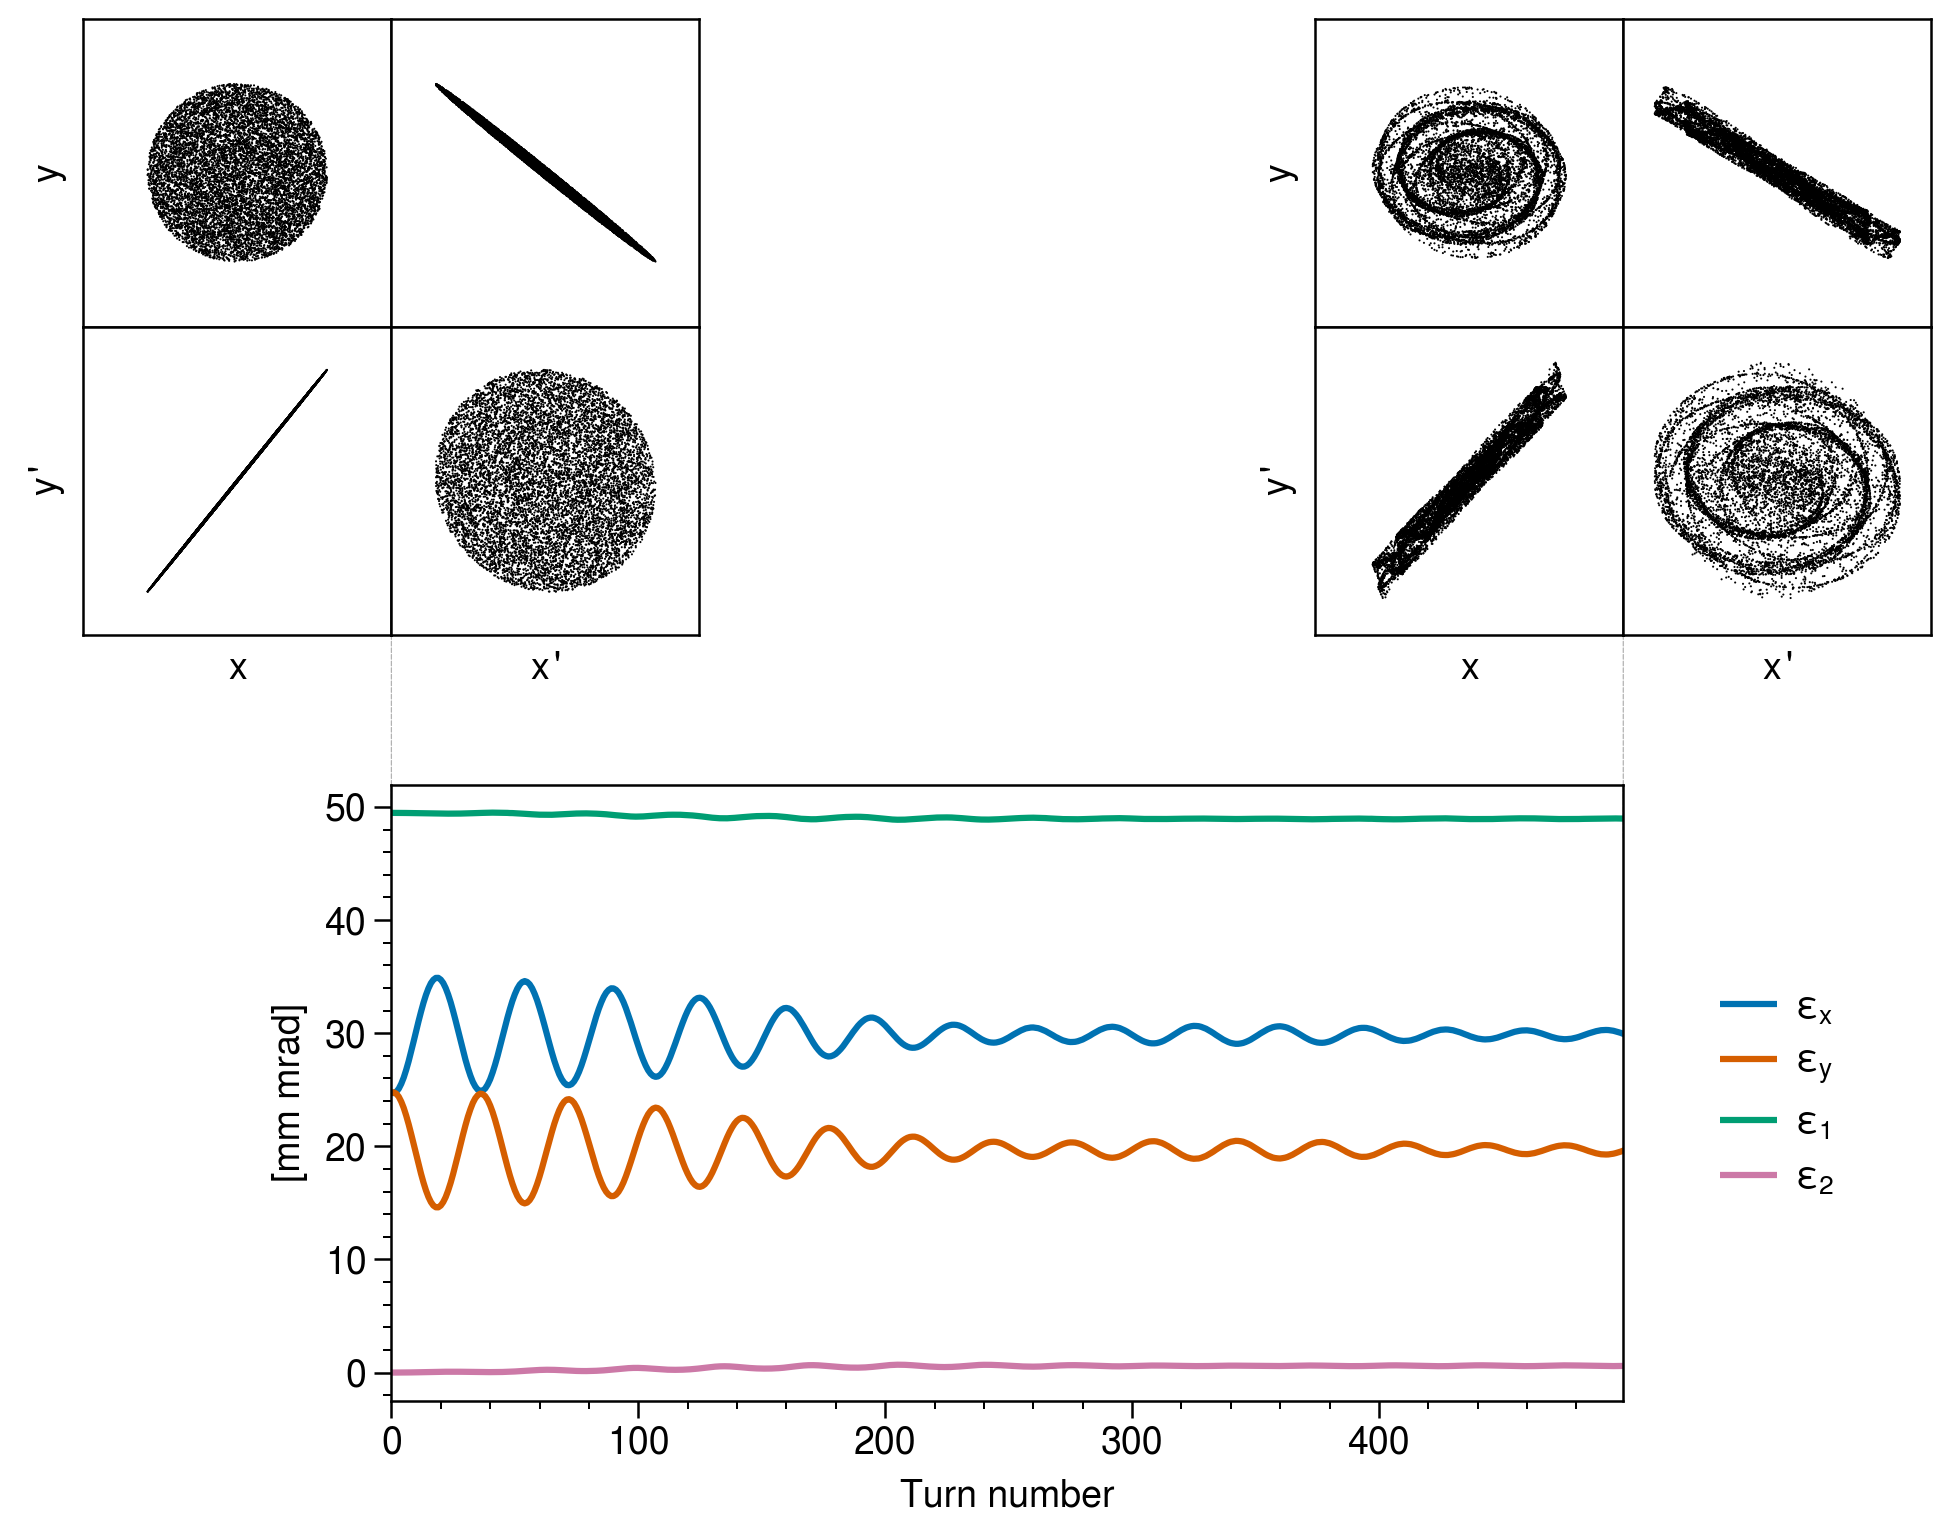
\includegraphics[width=0.7\textwidth]{Images/chapter3/fringe_solenoid.png}
    \caption{Danilov distribution tracked in the SNS ring with a solenoid added to the ring. Fringe fields are the only nonlinear external effect.}
    \label{fig:fringe_b}
    \vspace*{3cm}
\end{figure}

\begin{figure}[!p]
    \centering
    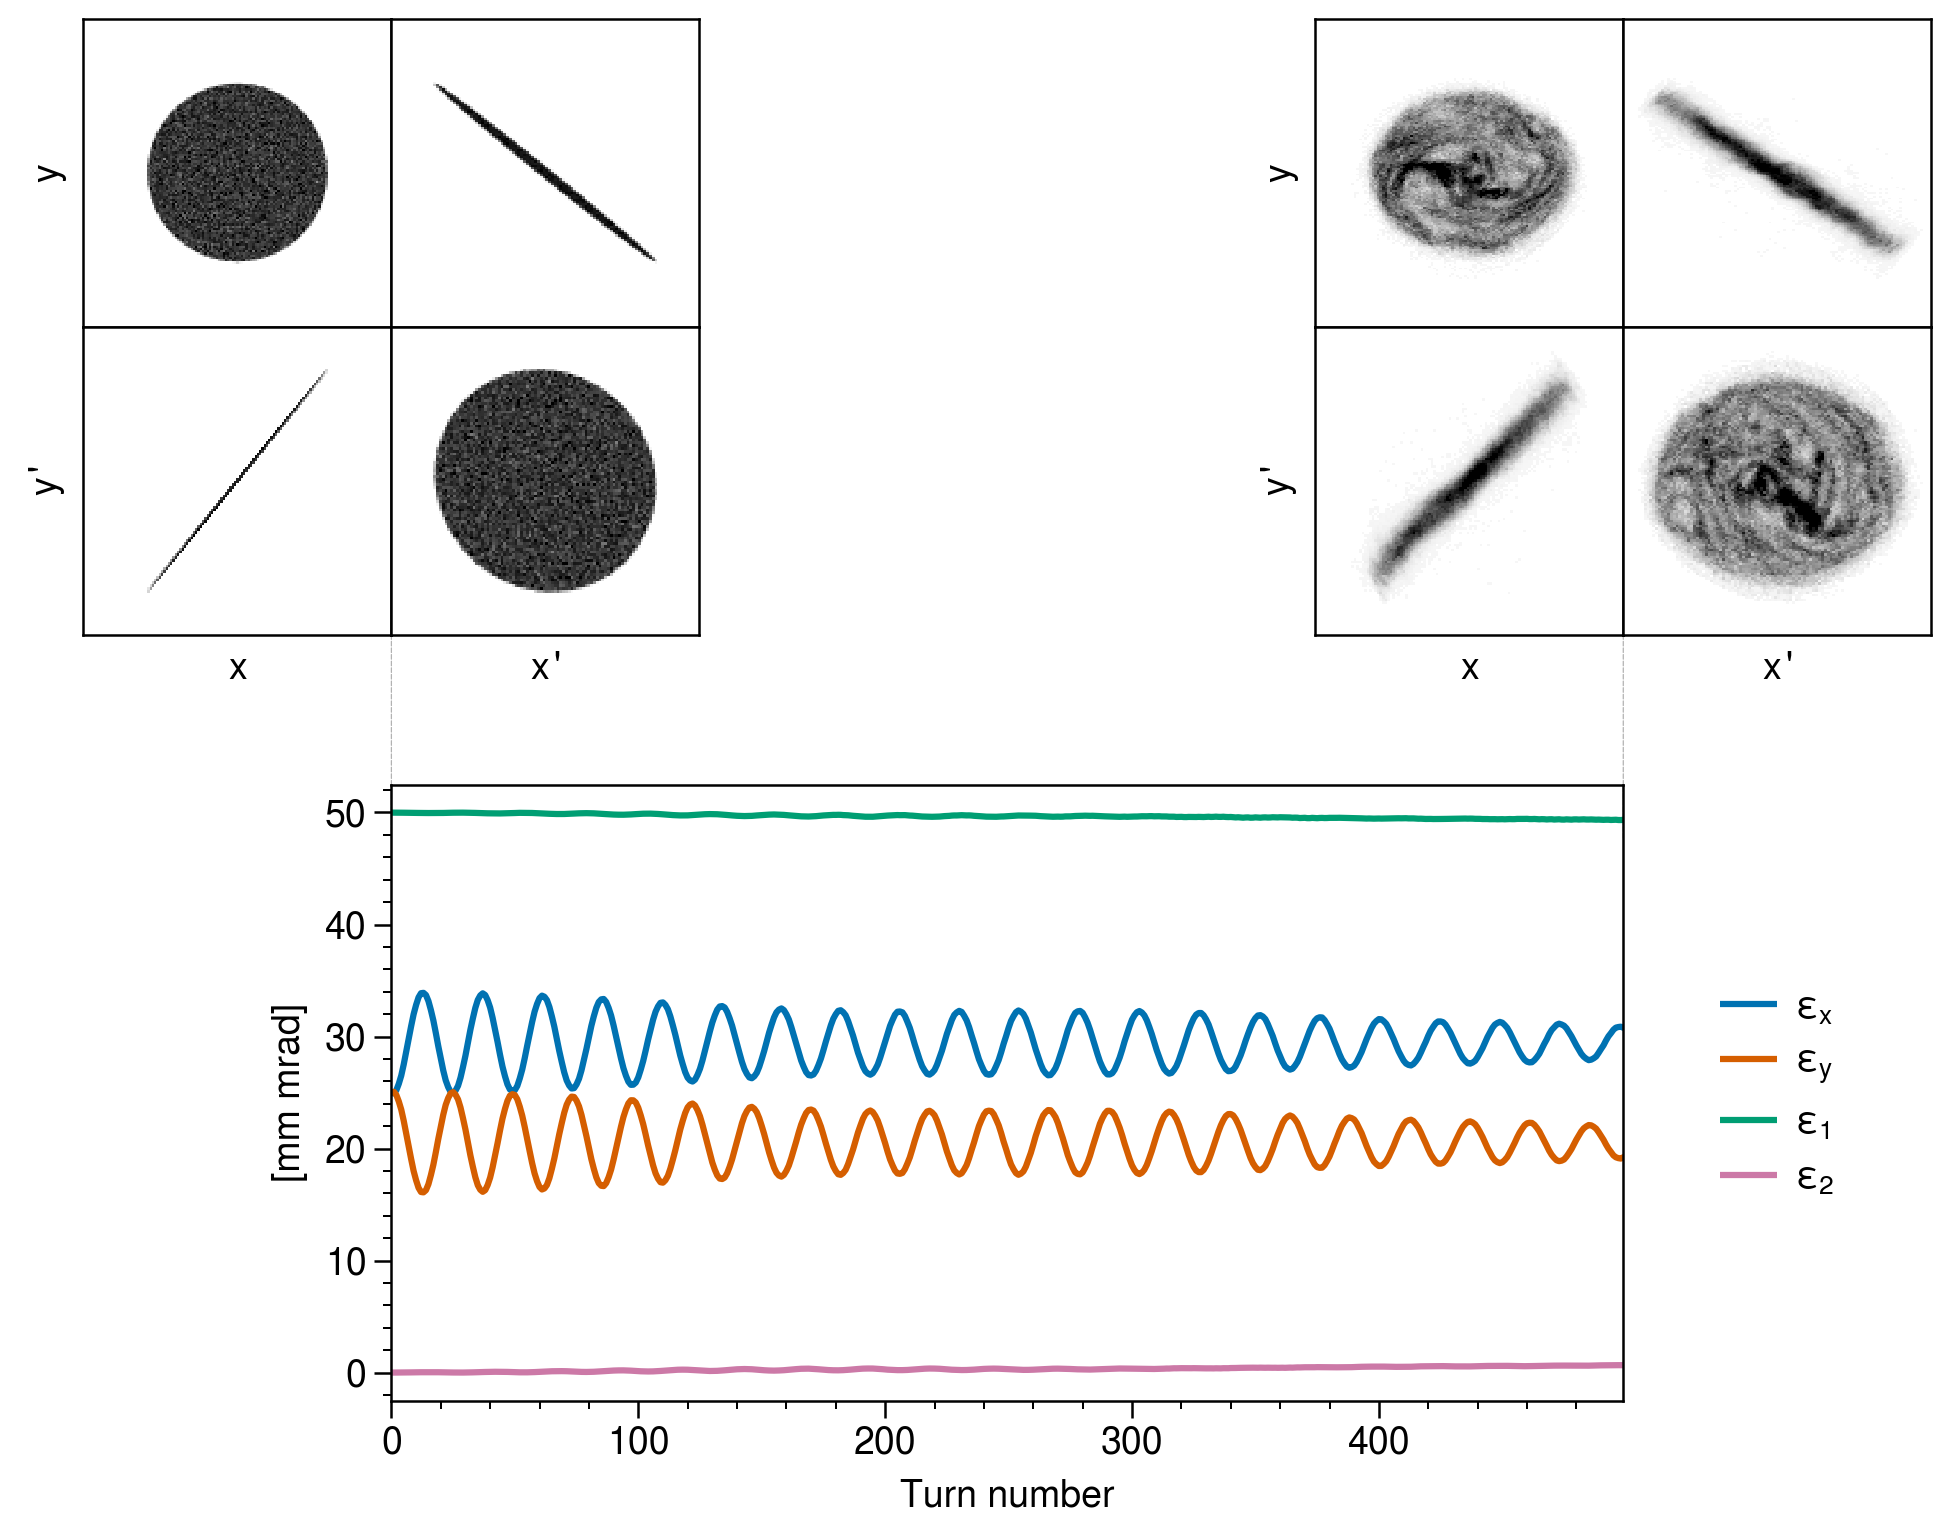
\includegraphics[width=0.7\textwidth]{Images/chapter3/fringe_spacecharge.png}
    \caption{Danilov distribution tracked in the SNS ring with space charge. Fringe fields are the only nonlinear external effect.}
    \label{fig:fringe_c}
    \vspace*{3cm}
\end{figure}

There is nonlinear coupling between the horizontal and vertical motion, and the final distribution is a superposition of rotating and counter-rotating modes. In Fig.~\ref{fig:fringe_b}, a solenoid magnet is added to the ring. The cross-plane correlations are now mostly maintained. The tunes $\nu_{1, 2}$ are no longer equal due to the linear coupling from the solenoid, so the resonance condition is avoided. In Fig.~\ref{fig:fringe_c}, the simulation is repeated with the inclusion of space charge instead of the solenoid magnet. An intensity of $10^{14}$ is used and the bunch length is equal to the ring length. It appears that a Danilov distribution will self-stabilize against the difference resonance when space charge is included.

It is recommended, however, that solenoid magnets be added to the ring to carry out this painting scheme. The difficulty is that the fringe fields dominate at the beginning of injection, when the transverse displacement is maximum, before space charge has a chance to stabilize the beam. Additionally, without a solenoid in the ring, the quality of the final distribution is very sensitive to the difference in horizontal and vertical tunes. With a solenoid in the ring, elliptical trajectories at the injection point are produced no matter the original horizontal and vertical tunes. 